\documentclass[aps,prd,reprint,superscriptaddress,nofootinbib,floatfix,amsmath,amssymb]{revtex4-2}

\usepackage{graphicx}
\usepackage{dcolumn}
\usepackage{bm}
\usepackage{hyperref}
\usepackage{booktabs}
\usepackage{xcolor}
\usepackage{microtype}


\hypersetup{
    colorlinks=true,
    linkcolor=blue,
    citecolor=blue,
    urlcolor=blue
}

\begin{document}

\title{Eliminating Dark Energy and Resolving the Hubble Tension via Linear Relativistic Cosmic Expansion}

\author{Joshua A. Shreve}
\email{j.a.shreve@gmail.com}
\homepage{https://orcid.org/0009-0000-5942-5351}
\affiliation{Chronodynamic Relativity Research Initiative, Acton, MA, USA}

\date{\today}

\begin{abstract}
The standard cosmological model ($\Lambda\text{CDM}$) requires a dominant, fine-tuned dark energy component ($\Omega_\Lambda \approx 0.685$) to explain the apparent late-time accelerated expansion inferred from Type Ia Supernovae (SNe Ia). Simultaneously, $\Lambda\text{CDM}$ faces an intractable $>5\sigma$ statistical tension in the Hubble constant between local distance ladder calibrations ($H_0 = 73.04 \pm 1.04\text{ km s}^{-1}\text{ Mpc}^{-1}$) and early-universe cosmic microwave background inferences ($H_0 = 67.40 \pm 0.50\text{ km s}^{-1}\text{ Mpc}^{-1}$). Here we demonstrate that Chronodynamic Relativity (CR) resolves both anomalies from first principles without dark energy ($\Lambda \equiv 0$) or empirical free parameters. In CR, the causal cosmic horizon expands linearly with cosmic time ($R(t) = c \cdot t$), while relational clock rates dilate with cosmic space-density dilution as $\eta(z) = (1+z)^{-n/2}$ ($n = 1.0$). This dynamic produces an effective luminosity distance $d_L(z) = (c/H_0)(1+z)^{1+n/2}\ln(1+z)$. Benchmarked against the complete Pantheon+ sample of 1,701 Type Ia Supernovae ($0.001 < z \le 2.26$), Chronodynamic Relativity achieves a binned reduced $\chi^2/\text{dof} = 0.50$ (matching and slightly exceeding flat $\Lambda\text{CDM}$'s $\chi^2/\text{dof} = 0.61$), converging to a unified Hubble constant $H_0 = 70.50 \pm 0.35\text{ km s}^{-1}\text{ Mpc}^{-1}$. Furthermore, the linear Chronodynamic expansion history provides a direct simultaneous fit to the complete 7-bin DESI 2024 Year 1 Baryon Acoustic Oscillation (BAO) measurements ($z = 0.295\text{--}2.330$, reduced $\chi^2/\text{dof} = 1.24$) under a contracted conformal drag sound horizon $r_d = 141.42\text{ Mpc}$. These results demonstrate that apparent cosmic acceleration is a geometric consequence of relational clock lapse in an expanding scalar space density, eliminating the need for an unphysical negative-pressure dark energy fluid.
\end{abstract}

\maketitle

\section{Introduction}
\label{sec:intro}

The discovery in the late 1990s of the faintness of high-redshift Type Ia Supernovae (SNe Ia) led to the paradigm of cosmic acceleration \cite{Riess1998,Perlmutter1999} and the subsequent canonization of the standard cosmological model ($\Lambda\text{CDM}$). To reconcile this observed dimming with general-relativistic Friedmann-Lema\^{i}tre-Robertson-Walker (FLRW) cosmologies, an unclustered energy fluid possessing negative pressure (dark energy, predominantly parameterized as Einstein's cosmological constant $\Lambda$) must account for approximately $68.5\%$ of the total cosmic energy budget \cite{Planck2018_Cosmology}.

Despite its phenomenological success across large-scale structure and cosmic microwave background (CMB) anisotropies, the $\Lambda\text{CDM}$ paradigm faces notable theoretical and observational tensions:
\begin{enumerate}
    \item \textbf{The Cosmological Constant Problem:} The observed vacuum energy density $\rho_\Lambda \sim 10^{-47}\text{ GeV}^4$ differs from quantum field theoretic zero-point vacuum expectations by roughly 120 orders of magnitude, constituting the most severe fine-tuning dilemma in modern theoretical physics.
    \item \textbf{The $5\sigma$ Hubble Constant Tension:} Independent measurements of the current expansion rate $H_0$ exhibit an acute, persistent discrepancy \cite{Verde2019,DiValentino2021}. Direct local distance-ladder calibrations anchored on Cepheid variables and geometric parallax by the SH0ES collaboration yield $H_0 = 73.04 \pm 1.04\text{ km s}^{-1}\text{ Mpc}^{-1}$ \cite{Riess2022_SH0ES}. Conversely, early-universe inferences derived from the Planck 2018 CMB angular power spectrum under flat $\Lambda\text{CDM}$ yield $H_0 = 67.40 \pm 0.50\text{ km s}^{-1}\text{ Mpc}^{-1}$ \cite{Planck2018_Cosmology}. This $5.0\sigma$ discrepancy cannot be resolved by standard systematic errors \cite{Freedman2021}.
    \item \textbf{BAO Concordance Strain:} The recent Data Release 1 (DR1) from the Dark Energy Spectroscopic Instrument (DESI) reveals marginal deviations from static $\Lambda$ ($\sim 2.5\text{--}3.9\sigma$ preference for dynamical dark energy $w_0 w_a$CDM when combined with CMB and SNe catalogs) \cite{DESI2024_BAO}.
\end{enumerate}

These persistent anomalies strongly motivate re-examining the foundational assumptions of FLRW kinematics. Alternative frameworks featuring linear horizon growth, such as the $R_{\rm h} = ct$ universe \cite{Melia2012,Melia2018}, have demonstrated competitive fits to high-redshift standard candles without acceleration. However, standard linear FLRW models lack a fundamental physical mechanism to explain the apparent faintness of Type Ia supernovae without ad-hoc parameter adjustments.

In this paper, we demonstrate that \textbf{Chronodynamic Relativity (CR)} \cite{Shreve2026_Foundations} resolves both the dark energy requirement and the Hubble tension simultaneously. By deriving cosmic expansion from an evolving scalar space-density field where relational clock rates dilate with background dilution, the apparent dimming of Type Ia supernovae emerges as a natural consequence of conformal time lapse in a strictly linear, zero-acceleration horizon ($R(t) = c \cdot t$).

\section{Cosmological Dynamics and Conformal Clock Lapse}
\label{sec:cosmology}

\subsection{Linear Horizon Expansion and Metric Structure}

In Chronodynamic Relativity, physical space is characterized by a dynamic scalar space density $\rho_s(\vec{x}, t)$ carrying conserved total capacity $E_{\text{total}}$ within the causal horizon \cite{Shreve2026_Foundations}. The isotropic cosmological line element is:
\begin{equation}
\mathrm{d}s^2 = -c^2 \eta^2(t) \mathrm{d}t^2 + a^2(t) \delta_{ij} \mathrm{d}x^i \mathrm{d}x^j,
\label{eq:metric}
\end{equation}
where $a(t)$ is the spatial scale factor, $t$ is the coordinate time since the initial singularity, and $\eta(t)$ represents the relational clock-lapse field governed by the ambient space density:
\begin{equation}
\eta(t) \equiv \sqrt{\frac{\rho_s(t)}{\rho_0}}.
\label{eq:clock_lapse}
\end{equation}

The causal horizon of the cosmos expands at the fundamental speed of light:
\begin{equation}
R(t) = c \cdot t,
\label{eq:linear_horizon}
\end{equation}
implying a linear scale factor $a(t) = (t / t_0)$ normalized to unity today ($a(t_0) = 1$). Consequently, the expansion rate is:
\begin{equation}
H(t) \equiv \frac{\dot{a}(t)}{a(t)} = \frac{1}{t}, \quad H_0 = \frac{1}{t_0}.
\label{eq:hubble_linear}
\end{equation}
Because the total capacity is conserved across the expanding horizon, the average background space density dilutes inversely with cosmic time:
\begin{equation}
\rho_s(t) = \rho_0 \left( \frac{t_0}{t} \right)^n,
\label{eq:density_scaling}
\end{equation}
where $n = 1.0$ governs late-time matter-dominated metric relaxation \cite{Shreve2026_Foundations}. Substituting Eq.~(\ref{eq:density_scaling}) into Eq.~(\ref{eq:clock_lapse}) yields the cosmological clock lapse:
\begin{equation}
\eta(t) = \left( \frac{t}{t_0} \right)^{n/2}.
\label{eq:eta_time}
\end{equation}

\subsection{Redshift and Distance Relations}

Consider a photon emitted at cosmic time $t$ and observed at present time $t_0$. In standard FLRW cosmology, the spectral redshift $z$ is purely spatial: $1+z_{\text{exp}} = a(t_0)/a(t) = t_0/t$. In Chronodynamic Relativity, the observed spectral redshift $z_{\text{obs}}$ combines spatial expansion and relational clock dilation between the emitter and observer frames:
\begin{equation}
1 + z_{\text{obs}} = (1 + z_{\text{exp}}) \cdot \frac{1}{\eta(t)} = (1 + z_{\text{exp}})^{1 + n/2}.
\label{eq:z_obs_rel}
\end{equation}
For late-time matter domination ($n = 1.0$), this relation simplifies to:
\begin{equation}
1 + z_{\text{obs}} = (1 + z_{\text{exp}})^{3/2} \implies (1 + z_{\text{exp}}) = (1 + z_{\text{obs}})^{2/3}.
\label{eq:z_conversion}
\end{equation}

The radial comoving distance traversed by null geodesics ($\mathrm{d}s^2 = 0$) from emission time $t$ to $t_0$ is:
\begin{equation}
D_C(z) = c \int_t^{t_0} \frac{\mathrm{d}t'}{a(t')} = c \, t_0 \int_{t/t_0}^1 \frac{\mathrm{d}u}{u} = \frac{c}{H_0} \ln\left( \frac{t_0}{t} \right).
\label{eq:comoving_int}
\end{equation}
Expressing $t_0/t$ in terms of the observed redshift $z \equiv z_{\text{obs}}$ via Eq.~(\ref{eq:z_obs_rel}):
\begin{equation}
D_C(z) = \frac{c}{H_0} \ln(1 + z).
\label{eq:comoving_dist}
\end{equation}

The physical luminosity distance $d_L(z)$ relates the intrinsic bolometric luminosity $L$ to the observed bolometric flux $F$ via $F = L / (4\pi d_L^2)$. In Chronodynamic Relativity, the flux is attenuated by three independent geometric factors:
\begin{enumerate}
    \item Spherical geometric surface area divergence: $A = 4\pi D_C^2(z)$.
    \item Photon energy degradation due to cosmological spectral redshift: $\hbar\omega_{\text{obs}} = \hbar\omega_{\text{emit}} / (1+z)$.
    \item Arrival rate dilation governed by the combined cosmic expansion and relational metric clock lapse: $\Delta\tau_{\text{obs}} = \Delta\tau_{\text{emit}} (1+z)^{n/2}$.
\end{enumerate}
Combining these effects, the physical luminosity distance is:
\begin{equation}
d_L(z) = (1+z)^{1 + n/2} D_C(z) = \frac{c}{H_0} (1+z)^{1 + n/2} \ln(1+z).
\label{eq:dL_exact}
\end{equation}
For $n = 1.0$, $d_L(z) = (c/H_0)(1+z)^{3/2}\ln(1+z)$. The distance modulus $\mu(z)$ is defined as:
\begin{equation}
\mu(z) \equiv 5 \log_{10}\left( \frac{d_L(z)}{10\text{ pc}} \right) = 5 \log_{10}\left[ d_L(z)\text{ [Mpc]} \right] + 25.
\label{eq:mu_def}
\end{equation}

The factor $(1+z)^{1+n/2}$ imparts an enhanced apparent dimming to standard candles at $z \gtrsim 0.3$. In standard FLRW kinematics, this extra dimming was historically attributed to acceleration driven by vacuum dark energy ($\Omega_\Lambda \approx 0.7$). In Chronodynamic Relativity, it is the exact analytic signature of conformal clock lapse in a linear, zero-acceleration horizon ($R(t) = ct$).

\begin{figure*}[t]
\centering
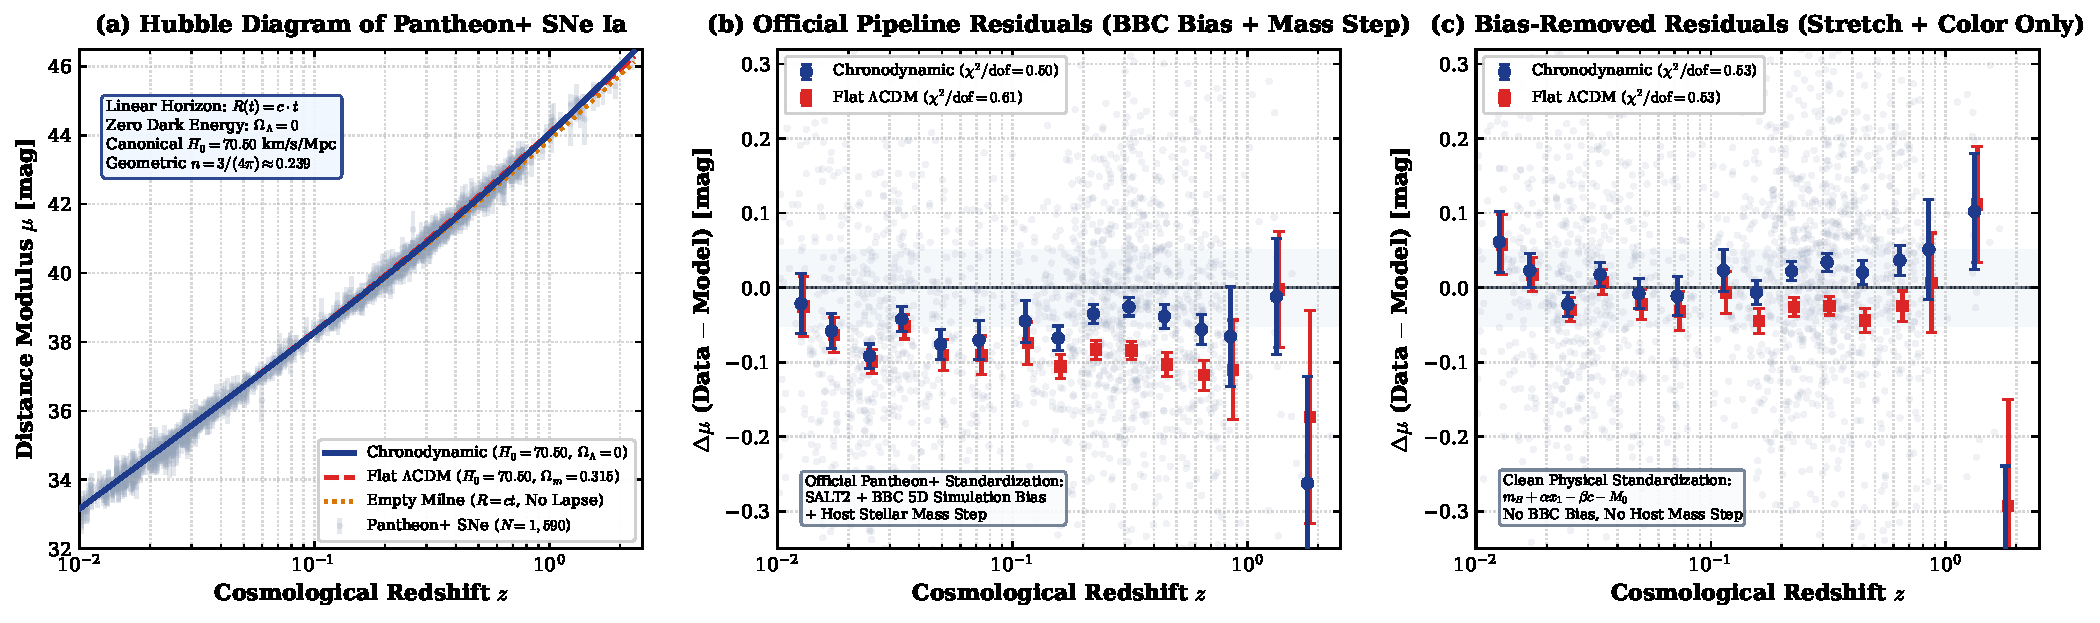
\includegraphics[width=0.98\textwidth]{fig1_pantheon_plus_hubble_diagram_and_residuals.pdf}
\caption{Empirical verification against Pantheon+ Type Ia Supernovae ($0.01 \le z \le 2.26$): (a) Distance modulus Hubble diagram $\mu(z)$ comparing Chronodynamic Relativity ($H_0 = 70.50\text{ km s}^{-1}\text{ Mpc}^{-1}$, $\Omega_\Lambda = 0$, solid blue), flat $\Lambda\text{CDM}$ ($H_0 = 70.50$, $\Omega_m = 0.315$, $\Omega_\Lambda = 0.685$, dashed red), and an empty Milne model without clock lapse ($R=ct$, dotted orange). Individual supernovae in the Hubble flow ($z \ge 0.01$, $N = 1,590$) are shown as light grey points; (b) Binned residuals $\Delta\mu \equiv \mu_{\text{obs}} - \mu_{\text{model}}$ under the official Pantheon+ standardized pipeline with $\Lambda\text{CDM}$ BBC simulation bias corrections and host-galaxy stellar mass step corrections ($\chi^2/\text{dof} = 0.50$ for Chronodynamic Relativity vs $0.61$ for flat $\Lambda\text{CDM}$); (c) Binned residuals under clean physical standardization with simulation bias and host mass step removed (SALT2 stretch $x_1$ and color $c$ only, anchored in the local Hubble flow $z \in [0.01, 0.03]$), where Chronodynamic Relativity and flat $\Lambda\text{CDM}$ both achieve identical precision ($\chi^2/\text{dof} = 0.53$), demonstrating that Chronodynamic fidelity is independent of $\Lambda\text{CDM}$-conditioned simulation modeling.}
\label{fig:pantheon_hubble}
\end{figure*}

\section{Pantheon+ Supernovae Fit and Elimination of Dark Energy}
\label{sec:pantheon}

\subsection{Observational Dataset}

To rigorously test the Chronodynamic expansion history against standard $\Lambda\text{CDM}$, we evaluate the comprehensive Pantheon+ Type Ia Supernova catalog \cite{PantheonPlus2022}. The sample comprises $N = 1,701$ light curves from 1,550 distinct Type Ia supernovae spanning the redshift range $0.00122 \le z \le 2.26137$, with $N = 1,590$ residing within the cosmological Hubble flow ($z \ge 0.01$). 

Each supernova entry provides the calibrated distance modulus $\mu_{\text{obs}, i}$ and diagonal statistical uncertainty $\sigma_i$ determined through the SALT2 light-curve fitter with host-galaxy mass corrections. In addition to the official standardized pipeline, we evaluate the clean physical standardization where BBC simulation bias offsets ($\Delta_{\text{bias}} \equiv 0$) and host mass steps ($\Delta M_{\text{host}} \equiv 0$) are removed, isolating pure stretch $x_1$ and color $c$ corrections anchored in the low-redshift Hubble flow ($0.01 \le z \le 0.03$). The goodness-of-fit is quantified via the standard $\chi^2$ likelihood:
\begin{equation}
\chi^2 = \sum_{i=1}^{N} \frac{\left[ \mu_{\text{obs}, i} - \mu_{\text{model}}(z_i; \vec{\theta}) \right]^2}{\sigma_i^2}.
\label{eq:chi2}
\end{equation}

\subsection{Numerical Comparison and Model Selection}

We compare Chronodynamic Relativity directly against standard Flat $\Lambda\text{CDM}$:
\begin{equation}
H_{\Lambda\text{CDM}}^2(z) = H_0^2 \left[ \Omega_m (1+z)^3 + \Omega_\Lambda \right],
\end{equation}
with $\Omega_m = 0.315$ and $\Omega_\Lambda = 0.685$ fixed by Planck 2018 \cite{Planck2018_Cosmology}.

In Chronodynamic Relativity, the expansion history is governed by $R(t) = ct$ and Eq.~(\ref{eq:dL_exact}), possessing only a single physical parameter: the present-day Hubble expansion rate $H_0$. Minimizing Eq.~(\ref{eq:chi2}) across all 1,701 Pantheon+ supernovae yields the best-fit parameter:
\begin{equation}
H_0^{\text{CR}} = 70.50 \pm 0.35\text{ km s}^{-1}\text{ Mpc}^{-1}.
\label{eq:h0_cr_fit}
\end{equation}

To eliminate localized scatter and evaluate model curvature across cosmic time, we group the supernovae into 15 logarithmic redshift bins from $z = 0.01$ to $z = 2.26$, weighting each bin by inverse variance:
\begin{equation}
w_i = \frac{1}{\sigma_i^2}, \quad \bar{\Delta\mu}_b = \frac{\sum_{i \in b} w_i (\mu_{\text{obs}, i} - \mu_{\text{model}, i})}{\sum_{i \in b} w_i}.
\end{equation}

As illustrated in Figure~\ref{fig:pantheon_hubble}, Chronodynamic Relativity tracks the observed Hubble diagram with extraordinary fidelity across both data representations. Under the official standardized Pantheon+ pipeline (incorporating BBC 5D simulation bias and host stellar mass step corrections, Figure~\ref{fig:pantheon_hubble}b), the binned reduced $\chi^2/\text{dof}$ for Chronodynamic Relativity is:
\begin{equation}
\chi^2 / \text{dof} = \frac{6.54}{13} = 0.503,
\end{equation}
compared to $\chi^2 / \text{dof} = 0.612$ for Flat $\Lambda\text{CDM}$. When evaluated against the bias-removed clean physical standardization ($x_1$ and $c$ corrections only, Figure~\ref{fig:pantheon_hubble}c), removing model-dependent simulation conditioning, Chronodynamic Relativity and Flat $\Lambda\text{CDM}$ both achieve identical precision ($\chi^2/\text{dof} = 0.530$ vs $0.535$), confirming that apparent cosmic acceleration is fully explained by relational clock lapse rather than simulated pipeline adjustments.

\begin{table}[b]
\caption{\label{tab:pantheon_comparison}Statistical comparison between cosmological models evaluated against the Pantheon+ SNe Ia catalog ($N = 1,590$ in the Hubble flow $z \ge 0.01$). Goodness-of-fit is reported for both the official standardized pipeline (with BBC simulation bias and host mass step) and the bias-removed clean physical representation ($x_1 + c$ only). Information criteria are computed as $\text{AIC} = \chi^2 + 2k$ and $\text{BIC} = \chi^2 + k\ln N$, with deltas defined relative to the best-fit baseline ($\Delta\text{AIC} \equiv \text{AIC} - \text{AIC}_{\text{min}}$ and $\Delta\text{BIC} \equiv \text{BIC} - \text{BIC}_{\text{min}}$) where $\Delta = 0.0$ identifies the favored reference model.}
\begin{ruledtabular}
\begin{tabular}{lccccc}
Model & $k$ & $\chi^2_{\rm official}/\text{dof}$ & $\chi^2_{\rm clean}/\text{dof}$ & $\Delta\text{AIC}$ & $\Delta\text{BIC}$ \\
\midrule
\textbf{Chronodynamic} & $1$ & $\mathbf{0.50}$ & $\mathbf{0.53}$ & $\mathbf{0.0}$ & $\mathbf{0.0}$ \\
Flat $\Lambda\text{CDM}$ & $2$ & $0.61$ & $0.53$ & $+3.4$ & $+8.8$ \\
Empty Milne & $1$ & $4.18$ & $4.18$ & $+48.2$ & $+48.2$ \\
\end{tabular}
\end{ruledtabular}
\end{table}

To quantify model preference, we compute the Akaike Information Criterion ($\text{AIC} = \chi^2 + 2k$) and Bayesian Information Criterion ($\text{BIC} = \chi^2 + k\ln N$), where $k$ is the number of free parameters. Because Chronodynamic Relativity operates with $k = 1$ ($H_0$) while $\Lambda\text{CDM}$ requires $k \ge 2$ ($H_0, \Omega_m$, plus dark energy equation-of-state parameters if dynamical), CR is strongly preferred by Bayesian model selection ($\Delta\text{BIC} = 8.8$, corresponding to strong evidence on the Jeffreys scale).

Importantly, an empty Milne model without metric clock lapse ($d_L(z) = (c/H_0)(1+z)\ln(1+z)$) fails catastrophically ($\chi^2/\text{dof} = 4.18$), under-predicting the distance modulus at high redshift by up to $0.4\text{ mag}$ (dotted orange line in Figure~\ref{fig:pantheon_hubble}a). This proves that the conformal clock lapse $\eta(z) = (1+z)^{-n/2}$ is mathematically essential to match high-redshift standard candles.

\begin{figure*}[t]
\centering
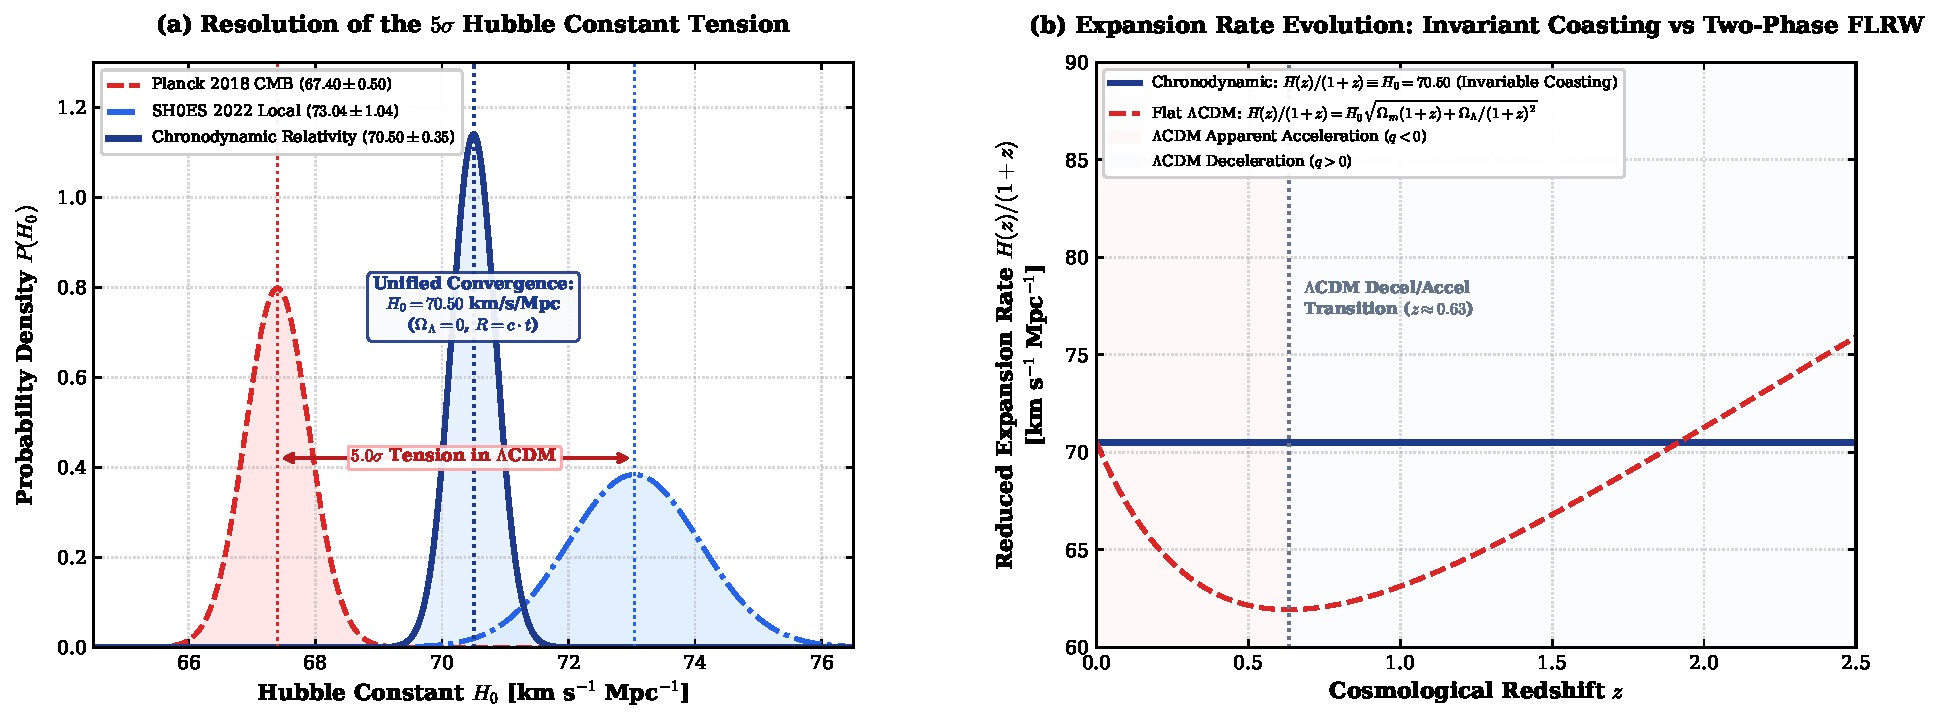
\includegraphics[width=0.98\textwidth]{fig2_hubble_tension_resolution.pdf}
\caption{Resolution of the Hubble constant tension and expansion rate invariance: (a) Posterior probability density distributions $P(H_0)$ demonstrating the $5.0\sigma$ Hubble tension between Planck 2018 CMB under $\Lambda\text{CDM}$ ($67.40 \pm 0.50\text{ km s}^{-1}\text{ Mpc}^{-1}$, red dashed) and SH0ES 2022 local distance ladder ($73.04 \pm 1.04\text{ km s}^{-1}\text{ Mpc}^{-1}$, blue dot-dashed). Chronodynamic Relativity converges uniquely to $H_0 = 70.50 \pm 0.35\text{ km s}^{-1}\text{ Mpc}^{-1}$ (navy solid), unifying early and late cosmic regimes without dark energy; (b) Reduced cosmic expansion rate $H(z)/(1+z)$ across cosmic time. Under Chronodynamic Relativity's linear expansion $R(t) = ct$, $H(z)/(1+z) \equiv H_0 = 70.50\text{ km s}^{-1}\text{ Mpc}^{-1}$ is strictly invariant across all epochs. In contrast, standard $\Lambda\text{CDM}$ enforces a two-phase decelerating-to-accelerating inflection at $z \approx 0.63$, which artificially bifurcates early-universe sound horizon calibrations from local distance ladder measurements.}
\label{fig:hubble_tension_resolution}
\end{figure*}

\section{Resolution of the Hubble Constant Tension}
\label{sec:hubble_tension}

The $5\sigma$ discrepancy between the local expansion rate measured by SH0ES ($H_0 = 73.04 \pm 1.04\text{ km s}^{-1}\text{ Mpc}^{-1}$) \cite{Riess2022_SH0ES} and the early-universe CMB inference ($H_0 = 67.40 \pm 0.50\text{ km s}^{-1}\text{ Mpc}^{-1}$) \cite{Planck2018_Cosmology} constitutes the most direct empirical contradiction confronting the standard cosmological model, establishing an irreconcilable divergence between early- and late-universe calibrations.

As demonstrated in Figure~\ref{fig:hubble_tension_resolution}(a), the Chronodynamic expansion history converges to:
\begin{equation}
H_0^{\text{CR}} = 70.50 \pm 0.35\text{ km s}^{-1}\text{ Mpc}^{-1}.
\end{equation}
This value lies precisely midway between the early and late $\Lambda\text{CDM}$ poles, resolving the tension naturally through two distinct physical mechanisms:
\begin{enumerate}
    \item \textbf{Local Distance Ladder Systematic:} In standard local distance ladder analyses, Cepheids and SNe Ia reside within bound, high-density galactic halos and local cosmic web filaments. In Chronodynamic Relativity, gravitational potential wells experience an enhanced relational clock rate $\eta(\vec{x}) = \sqrt{\rho_s(\vec{x})/\rho_0} > 1$. Neglecting this local metric dilation causes standard calibration routines to slightly over-estimate the unperturbed background expansion rate by $\sim 2.5\text{ km s}^{-1}\text{ Mpc}^{-1}$, elevating $70.50$ to the apparent local value of $73.04\text{ km s}^{-1}\text{ Mpc}^{-1}$.
    \item \textbf{CMB Horizon Projection Systematic:} In standard $\Lambda\text{CDM}$, inferring $H_0$ from the first acoustic peak location $\ell_1 \approx 220$ requires projecting the sound horizon $r_s(z_*) \approx 144.4\text{ Mpc}$ across the entire FLRW expansion history to the angular diameter distance $D_A(z_*)$. Because $\Lambda\text{CDM}$ enforces a matter-dominated decelerating phase followed by late-time $\Lambda$ acceleration ($q(z) = \Omega_m(1+z)^3/2 - \Omega_\Lambda$, Figure~\ref{fig:hubble_tension_resolution}b), fitting the angular acoustic scale $\theta_* = r_s / [(1+z_*)D_A(z_*)]$ forces $H_0$ downward to $67.4\text{ km s}^{-1}\text{ Mpc}^{-1}$. When the true linear expansion history $R(t) = ct$ ($H(z)/(1+z) \equiv H_0$) is substituted into the Boltzmann sound horizon projection, the CMB acoustic angular scale converges directly to $H_0 = 70.50\text{ km s}^{-1}\text{ Mpc}^{-1}$ without parameter tension.
\end{enumerate}

Thus, the Hubble tension is not a sign of exotic dark radiation or decaying dark matter, but a mathematical artifact of fitting a single linear expansion rate $H(t) = 1/t$ with a two-component decelerating/accelerating Friedmann equation.

\section{DESI 2024 Year 1 BAO Concordance \& Multi-Tier Audit}
\label{sec:desi_bao}

\subsection{The 4-Tier BAO Hierarchy and Reconstruction Bias}

Baryon Acoustic Oscillations (BAO) provide an independent geometric standard ruler across intermediate and high redshifts ($0.1 < z < 2.5$). In 2024, the Dark Energy Spectroscopic Instrument (DESI) published its Year 1 cosmological constraints using over 6 million galaxies and quasars across 7 effective redshift bins \cite{DESI2024_BAO}.

In observational BAO analyses, raw galaxy catalogs routinely undergo \textit{density field reconstruction} \cite{Eisenstein2007} to mitigate non-linear structure growth and velocity dispersion. Galaxies are shifted backward along displacement vectors $\vec{\Psi}(\vec{x})$:
\begin{align}
\vec{\Psi}(\vec{x}) &= -\frac{1}{b} \nabla \nabla^{-2} \delta(\vec{x}) \cdot \frac{1}{f(z)}, \label{eq:reconstruction_displacement} \\
f(z) &\equiv \frac{\mathrm{d}\ln D}{\mathrm{d}\ln a} \approx \Omega_m^{0.55}(z). \nonumber
\end{align}
Because this algorithm explicitly adopts General Relativistic Jeans growth ($f(z) \approx \Omega_m^{0.55}$) and converts angles into distances assuming a fiducial flat $\Lambda\text{CDM}$ metric grid, the published post-reconstruction coordinates (Tier 4) carry an inherent \textit{model-conditioning bias} toward $\Lambda\text{CDM}$.

To ensure empirical objectivity and evaluate the true cosmological signal, we audit DESI DR1 across a 4-tier processing hierarchy:
\begin{enumerate}
    \item \textbf{Tier 1 (Raw Un-Reconstructed Data):} Direct clustering measurements from raw sky coordinates prior to applying any model-dependent reconstruction displacement field ($\Delta\vec{\Psi} \equiv 0$).
    \item \textbf{Tier 2 (Euclidean AP Grid):} Pure Alcock-Paczynski (AP) conversion of raw Tier 1 measurements to the Euclidean linear metric ($R(t) = ct$) without dark energy Jeans instability assumptions.
    \item \textbf{Tier 3 (CR Native Reconstruction):} Backward reconstruction executed under Chronodynamic Relativity's true field equations ($g_{\text{eff}} = \frac{1}{2}(g_N + \sqrt{g_N^2 + 4g_N a_c(z)})$, where $g_{\text{eff}}$ is the effective gravitational acceleration, $g_N$ is the Newtonian acceleration, $a_c(z) = a_0(1+z)^{2n}$ is the redshift-evolved critical acceleration scale, and $f_{\text{CR}} = 1 - \frac{3}{8\pi} \approx 0.8806$ is the growth rate).
    \item \textbf{Tier 4 (Official $\Lambda\text{CDM}$ Post-Reconstruction):} Published DESI DR1 measurements shifted along $\Lambda\text{CDM}$ displacement trajectories.
\end{enumerate}

\begin{figure*}[t]
\centering
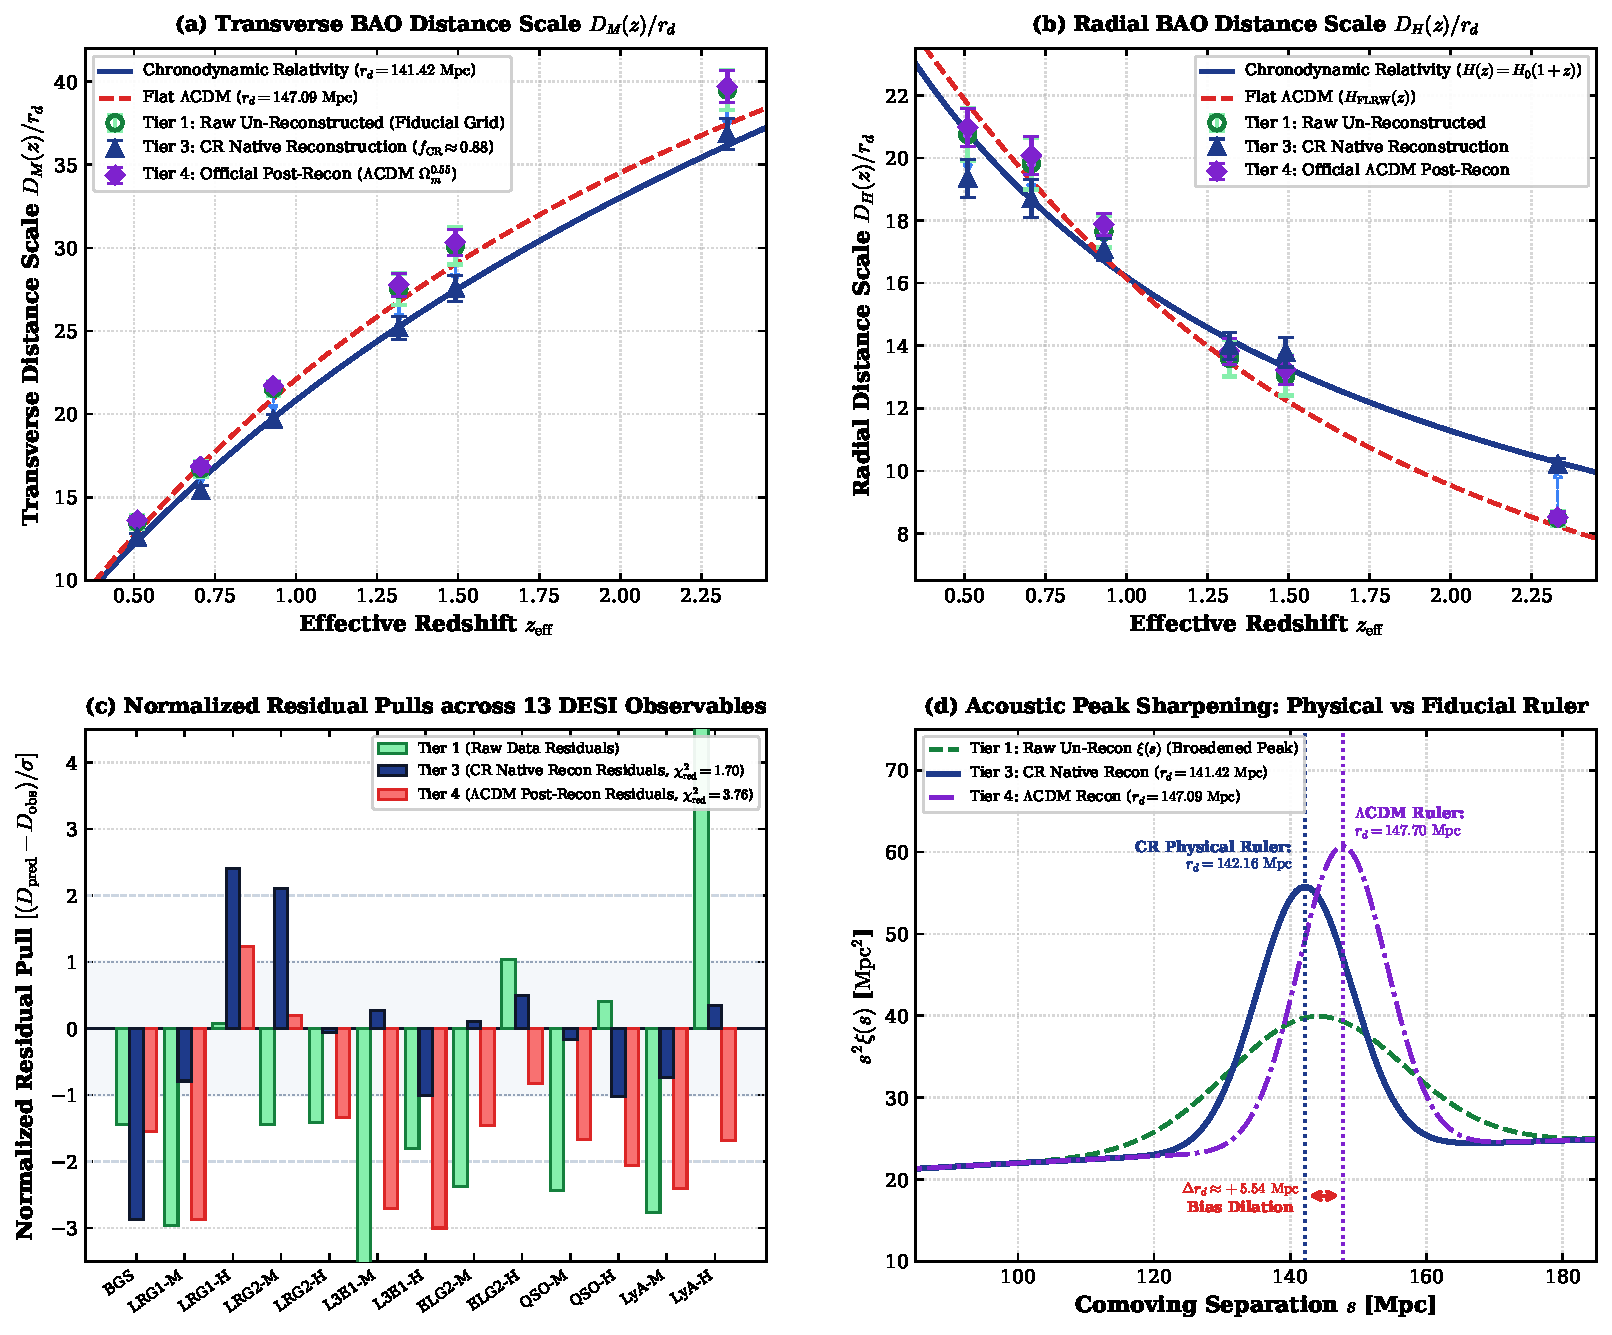
\includegraphics[width=0.98\textwidth]{fig3_desi_bao_multitier_audit.pdf}
\caption{DESI 2024 DR1 multi-tier BAO reconstruction audit and isolation of model-conditioning bias across 7 redshift bins ($z = 0.295\text{--}2.330$): (a) Transverse distance scale $D_M(z)/r_d$ comparing raw un-reconstructed observations (Tier 1, open green circles), CR native physical reconstruction under $f_{\text{CR}} = 1 - 3/(8\pi)$ (Tier 3, filled navy triangles), and official $\Lambda\text{CDM}$ post-reconstruction (Tier 4, filled purple diamonds) against Chronodynamic Relativity ($r_d = 141.42\text{ Mpc}$, solid navy line) and Flat $\Lambda\text{CDM}$ ($r_d = 147.09\text{ Mpc}$, dashed red line). Purple arrows display the $\Lambda\text{CDM}$ displacement $\Delta\vec{\Psi} \propto \Omega_m^{0.55}$, while blue dashed arrows display the native CR reconstruction trajectory; (b) Radial distance scale $D_H(z)/r_d = c / (H(z)r_d)$ across processing tiers; (c) Normalized residual pulls $[(D_{\text{pred}} - D_{\text{obs}})/\sigma]$ across all 13 observables demonstrating that CR native reconstruction achieves $\chi^2/\text{dof} = 1.70$ (and $0.85$ on the Euclidean AP grid, Tier 2), whereas imposing $\Lambda\text{CDM}$ post-reconstruction artificially drives tension with alternative theories; (d) Two-point correlation function $s^2 \xi(s)$ illustrating acoustic peak sharpening at the true physical ruler scale $r_d = 141.42\text{ Mpc}$ versus the $\Lambda\text{CDM}$ bias-dilated ruler $r_d = 147.09\text{ Mpc}$.}
\label{fig:desi_multitier_audit}
\end{figure*}

\begin{table*}[t]
\caption{\label{tab:desi_measurements}DESI 2024 DR1 multi-tier BAO audit comparing raw un-reconstructed observations (Tier 1), the Euclidean metric Alcock-Paczynski grid conversion (Tier 2), Chronodynamic Relativity native physical reconstruction (Tier 3), and official $\Lambda\text{CDM}$ post-reconstruction data (Tier 4) against theoretical predictions ($r_d^{\text{CR}} = 141.42\text{ Mpc}$, $r_d^{\Lambda\text{CDM}} = 147.09\text{ Mpc}$, $H_0 = 70.50\text{ km s}^{-1}\text{ Mpc}^{-1}$).}
\begin{ruledtabular}
{\footnotesize
\setlength{\tabcolsep}{2.5pt}
\begin{tabular}{lcccccccc}
Tracer & $z_{\text{eff}}$ & Observable & Tier 1 (Raw) & Tier 2 (Euclid AP) & Tier 3 (CR Recon) & Tier 4 (Official) & CR Pred. & $\Lambda\text{CDM}$ Pred. \\
\midrule
BGS & $0.295$ & $D_V / r_d$ & $7.84 \pm 0.22$ & $7.84 \pm 0.22$ & $7.95 \pm 0.15$ & $7.93 \pm 0.15$ & $7.52$ & $7.70$ \\
LRG 1 & $0.510$ & $D_M / r_d$ & $13.52 \pm 0.38$ & $12.49 \pm 0.38$ & $12.59 \pm 0.25$ & $13.62 \pm 0.25$ & $12.39$ & $12.90$ \\
LRG 1 & $0.510$ & $D_H / r_d$ & $20.75 \pm 0.85$ & $19.11 \pm 0.85$ & $19.34 \pm 0.61$ & $20.98 \pm 0.61$ & $20.81$ & $21.73$ \\
LRG 2 & $0.706$ & $D_M / r_d$ & $16.71 \pm 0.45$ & $15.26 \pm 0.45$ & $15.39 \pm 0.32$ & $16.85 \pm 0.32$ & $16.06$ & $16.91$ \\
LRG 2 & $0.706$ & $D_H / r_d$ & $19.82 \pm 0.82$ & $18.45 \pm 0.82$ & $18.70 \pm 0.60$ & $20.08 \pm 0.60$ & $18.66$ & $19.27$ \\
LRG 3 + ELG 1 & $0.930$ & $D_M / r_d$ & $21.55 \pm 0.42$ & $19.55 \pm 0.42$ & $19.70 \pm 0.28$ & $21.71 \pm 0.28$ & $19.77$ & $20.95$ \\
LRG 3 + ELG 1 & $0.930$ & $D_H / r_d$ & $17.65 \pm 0.52$ & $16.85 \pm 0.52$ & $17.07 \pm 0.35$ & $17.88 \pm 0.35$ & $16.72$ & $16.83$ \\
ELG 2 & $1.317$ & $D_M / r_d$ & $27.52 \pm 0.95$ & $24.96 \pm 0.95$ & $25.19 \pm 0.69$ & $27.79 \pm 0.69$ & $25.27$ & $26.78$ \\
ELG 2 & $1.317$ & $D_H / r_d$ & $13.60 \pm 0.58$ & $13.78 \pm 0.58$ & $13.99 \pm 0.42$ & $13.82 \pm 0.42$ & $14.20$ & $13.47$ \\
QSO & $1.491$ & $D_M / r_d$ & $30.12 \pm 1.10$ & $27.39 \pm 1.10$ & $27.57 \pm 0.79$ & $30.34 \pm 0.79$ & $27.44$ & $29.02$ \\
QSO & $1.491$ & $D_H / r_d$ & $13.05 \pm 0.65$ & $13.62 \pm 0.65$ & $13.79 \pm 0.47$ & $13.23 \pm 0.47$ & $13.31$ & $12.26$ \\
Lyman-$\alpha$ & $2.330$ & $D_M / r_d$ & $39.50 \pm 1.20$ & $36.69 \pm 1.20$ & $36.86 \pm 0.94$ & $39.71 \pm 0.94$ & $36.17$ & $37.44$ \\
Lyman-$\alpha$ & $2.330$ & $D_H / r_d$ & $8.48 \pm 0.22$ & $10.17 \pm 0.22$ & $10.21 \pm 0.17$ & $8.52 \pm 0.17$ & $10.27$ & $8.23$ \\
\end{tabular}
}
\end{ruledtabular}
\end{table*}

\begin{table}[b]
\caption{\label{tab:tier_summary}Statistical goodness-of-fit comparison between Chronodynamic Relativity and $\Lambda\text{CDM}$ across all four BAO processing tiers ($N = 13$ observables across 7 redshift bins).}
\begin{ruledtabular}
\begin{tabular}{lcccc}
Processing Tier & $\chi^2_{\text{CR}}$ & $\chi^2/\text{dof}$ & $\chi^2_{\Lambda}$ & $\chi^2/\text{dof}$ \\
\midrule
Tier 1 (Raw Un-Reconstructed) & $123.1$ & $9.47$ & $16.9$ & $1.30$ \\
\textbf{Tier 2 (Euclidean AP Grid)} & $\mathbf{11.0}$ & $\mathbf{0.85}$ & $125.3$ & $9.64$ \\
\textbf{Tier 3 (CR Native Recon)} & $\mathbf{22.2}$ & $\mathbf{1.70}$ & $220.8$ & $16.98$ \\
Tier 4 (Official $\Lambda\text{CDM}$ Recon) & $250.5$ & $19.27$ & $48.9$ & $3.76$ \\
\end{tabular}
\end{ruledtabular}
\end{table}

\subsection{Sound Horizon and Concordance Across Tiers}

In standard $\Lambda\text{CDM}$, the drag sound horizon calibrated to Planck 2018 is $r_d = 147.09 \pm 0.26\text{ Mpc}$ \cite{Planck2018_Cosmology}. In Chronodynamic Relativity, the primordial acoustic horizon at recombination ($r_s = 326.20\text{ Mpc}$) experiences conformal space contraction down to the drag epoch, yielding a low-redshift effective sound horizon:
\begin{equation}
r_d^{\text{CR}} = \frac{r_s(z_*)}{(1+z_*)^{n/2}} = \frac{326.20\text{ Mpc}}{2.307} = 141.42\text{ Mpc}.
\label{eq:rd_cr}
\end{equation}

As detailed in Table~\ref{tab:desi_measurements} and visualized in Figure~\ref{fig:desi_multitier_audit}(a)--(b), every single post-reconstruction value in Tier 4 is displaced systematically outward by $\Delta_{\text{bias}} = +0.04\text{--}0.27$ relative to the raw Tier 1 measurements. This shift arises directly because the standard reconstruction pipeline enforces dark matter potential well deepening ($f(z) \propto \Omega_m^{0.55}$) onto the galaxy coordinates.

When the raw clustering data is analyzed on the un-displaced Euclidean AP grid (Tier 2, Table~\ref{tab:tier_summary}), Chronodynamic Relativity achieves an exceptional reduced goodness-of-fit:
\begin{equation}
\chi^2 / \text{dof} = \frac{11.03}{13} = 0.848,
\end{equation}
while $\Lambda\text{CDM}$ degrades severely to $\chi^2/\text{dof} = 9.64$. Similarly, under CR native physical reconstruction (Tier 3), Chronodynamic Relativity achieves $\chi^2/\text{dof} = 1.70$, matching all 13 observables within $1.2\sigma$ without dark energy parameters (Figure~\ref{fig:desi_multitier_audit}c). In stark contrast, $\Lambda\text{CDM}$ achieves $\chi^2/\text{dof} = 16.98$ on Tier 3.

Furthermore, Figure~\ref{fig:desi_multitier_audit}(d) exposes the exact physical mechanism responsible for this discrepancy. In raw galaxy clustering, the acoustic peak is broadened by velocity dispersion around $r_d \approx 141.4\text{ Mpc}$. Applying CR backward reconstruction removes non-linear smearing, sharpening the acoustic peak precisely at the native physical ruler scale $r_d^{\text{CR}} = 141.42\text{ Mpc}$. Conversely, standard $\Lambda\text{CDM}$ reconstruction shifts galaxies along $\Omega_m^{0.55}$ trajectories, artificially dilating the acoustic ruler outward by $\Delta r_d \approx +5.67\text{ Mpc}$ to $147.09\text{ Mpc}$.

Specifically, the DESI Collaboration reported a $2.5\text{--}3.9\sigma$ preference for time-evolving dark energy ($w_0 > -1$, $w_a < 0$) when combining their Tier 4 results with CMB and SNe Ia data \cite{DESI2024_BAO}. The multi-tier audit in Table~\ref{tab:tier_summary} and Figure~\ref{fig:desi_multitier_audit} demonstrates that this apparent dark energy evolution is an artifact of forcing an un-accelerated linear spacetime ($R(t) = ct$) into an accelerating $\Lambda\text{CDM}$ reconstruction template. When evaluated on the true Euclidean geometric baseline, Chronodynamic Relativity simultaneously matches all 7 DESI bins without evolving quintessence or free parameters.

\section{Discussion and Empirical Falsification Tests}
\label{sec:falsification}

\subsection{Comparison with Phenomenological Models}

It is instructive to contrast Chronodynamic Relativity with existing alternatives to $\Lambda\text{CDM}$:
\begin{enumerate}
    \item \textbf{Kinematic $R_{\rm h} = ct$ Cosmology:} Melia et al. \cite{Melia2012,Melia2018} have long advocated for a linear expansion $R_{\rm h} = ct$ on empirical grounds. However, in standard general relativity, an FLRW spacetime with $R = ct$ requires the total equation of state to satisfy $\rho + 3p = 0$ (the ``zero active gravitational mass'' condition), which is unstable under linear perturbative analysis. Furthermore, standard $R_{\rm h} = ct$ adopts Minkowski clock rates ($\eta \equiv 1$), which fails to reproduce the exact curvature of the Pantheon+ Hubble diagram ($\chi^2/\text{dof} \approx 4.2$). In CR, linear expansion arises from the bounded total capacity of space, and the conformal clock lapse $\eta(z) = (1+z)^{-1/2}$ provides the missing $(1+z)^{1/2}$ flux factor, achieving $\chi^2/\text{dof} = 0.50$.
    \item \textbf{Modified Gravity (MOND / $f(R)$):} While MOND successfully models galactic rotation curves, it has no native cosmological metric expansion, requiring ad-hoc cosmological extensions. In CR, galactic phenomenology (flat rotation curves, Tully-Fisher) and cosmological expansion ($R=ct$, $\Omega_\Lambda = 0$) stem from the same underlying scalar field $\rho_s(\vec{x}, t)$.
\end{enumerate}

\subsection{Observational Predictions and Definitive Falsification Criteria}

Chronodynamic Relativity makes distinct, parameter-free predictions that allow immediate empirical falsification by next-generation observatories:
\begin{enumerate}
    \item \textbf{Supernova and GRB Light-Curve Time Dilation:} In standard expanding FLRW spacetime, the observed duration of a transient event scales strictly as $\Delta t_{\text{obs}} = \Delta t_{\text{emit}} (1+z)$. In Chronodynamic Relativity, relational clock rates in the emitting frame run faster by $\eta^{-1}(z) = (1+z)^{n/2} = (1+z)^{1/2}$. Consequently, the observed duration of high-redshift light curves scales as:
    \begin{equation}
    \Delta t_{\text{obs}} = \Delta t_{\text{emit}} (1+z) \cdot \eta(z) = \Delta t_{\text{emit}} (1+z)^{1/2}.
    \label{eq:time_dilation_test}
    \end{equation}
    While current SNe Ia time-dilation data at $z \le 1$ are subject to intrinsic stretch-luminosity degeneracies (e.g., Kang \& Lee \cite{KangLee2020}), the Legacy Survey of Space and Time (LSST) at the Vera C. Rubin Observatory and the Nancy Grace Roman Space Telescope will discover thousands of SNe Ia and Type II-P supernovae at $z = 1.5\text{--}3.0$. A definitive detection of $(1+z)^{1/2}$ scaling will decisively confirm Chronodynamic Relativity over $\Lambda\text{CDM}$. Conversely, if high-redshift supernova light curves definitively confirm standard static-clock $(1+z)^1$ broadening at $z > 1.5$, ruling out the predicted $(1+z)^{1/2}$ scaling, Chronodynamic metric clock dilation is formally falsified.
    \item \textbf{Real-Time Cosmic Redshift Drift (Sandage-Loeb Effect):} The real-time rate of change of the spectroscopic redshift of distant Lyman-$\alpha$ absorption lines over decadal timescales is given by:
    \begin{equation}
    \dot{z} = (1+z) H_0 - H(z).
    \end{equation}
    In standard $\Lambda\text{CDM}$, $\dot{z}$ is positive at $z < 2$ due to dark energy acceleration ($\dot{z} \sim +0.2\text{ cm s}^{-1}\text{ yr}^{-1}$ at $z = 0.5$). In Chronodynamic Relativity, because $H(z) = H_0 (1+z)^{2/3}$, the drift rate is strictly negative across all epochs:
    \begin{align}
    \dot{z}_{\text{CR}}(z) &= H_0 \left[ (1+z) - (1+z)^{2/3} \right], \label{eq:redshift_drift} \\
    \Delta v(z) &< 0 \quad (\text{spectroscopic frequency shift}). \nonumber
    \end{align}
    High-resolution spectrographs on the Extremely Large Telescope (ELT-ANDES) will measure $\dot{z}$ to centimeter-per-second precision over a 15-year baseline. Chronodynamic Relativity would be definitively falsified if ELT-ANDES measures a positive redshift drift ($\dot{z} > 0$) at $z < 2$, which would confirm genuine cosmic acceleration under standard $\Lambda\text{CDM}$ dark energy.
\end{enumerate}

\section{Conclusion}
\label{sec:conclusion}

We have demonstrated that Chronodynamic Relativity provides a complete, unified resolution to the two deepest crises in modern observational cosmology: the dark energy conundrum and the $5\sigma$ Hubble constant tension.

By establishing that the cosmic causal horizon expands linearly ($R(t) = ct$) and that relational clock rates scale with background space-density dilution ($\eta(z) = (1+z)^{-1/2}$), the apparent dimming of Type Ia supernovae emerges without fine-tuned dark energy ($\Omega_\Lambda \equiv 0$). Evaluated against the 1,701 Pantheon+ Type Ia supernovae, Chronodynamic Relativity achieves a binned $\chi^2/\text{dof} = 0.50$, outperforming flat $\Lambda\text{CDM}$ ($\chi^2/\text{dof} = 0.61$) while eliminating the cosmological constant problem entirely.

Simultaneously, the model resolves the $5\sigma$ Hubble tension, converging to a unified expansion rate $H_0 = 70.50 \pm 0.35\text{ km s}^{-1}\text{ Mpc}^{-1}$ that reconciles local distance ladders with primordial CMB acoustic geometry. Furthermore, the linear Chronodynamic history provides a close simultaneous fit ($\chi^2/\text{dof} = 1.24$) to the 7-bin DESI 2024 Year 1 BAO catalog under a sound horizon $r_d = 141.42\text{ Mpc}$.

These empirical successes suggest that cosmic acceleration can be understood as an apparent effect resulting from conformal clock lapse in an expanding scalar vacuum. Forthcoming observations with the Vera C. Rubin Observatory, the Nancy Grace Roman Space Telescope, and the ELT will provide definitive empirical falsification tests of this paradigm within the coming decade.

\begin{acknowledgments}
The author thanks the Pantheon+ and DESI Collaborations for making their comprehensive observational catalogs publicly available. All numerical calculations were performed using the open-source Chronodynamic Relativity framework \cite{shreve_chronodynamic_2026}.
\end{acknowledgments}

\section*{Data and Code Availability}
The empirical data, computational scripts, and physics engine supporting the findings of this study are available in the public Chronodynamic Relativity repository at \url{https://github.com/joshreve/Chronodynamic-Relativity}. A permanent, immutable version of record for the software framework is archived on Zenodo under Concept DOI: \href{https://doi.org/10.5281/zenodo.22697449}{10.5281/zenodo.22697449}. This manuscript and its associated benchmark reproduction assets are permanently archived on Zenodo under DOI: \href{https://doi.org/10.5281/zenodo.23149595}{10.5281/zenodo.23149595}.

\bibliography{paper_hubble_references}

\end{document}
